The NavIC simulator approach is as shown in figure \ref{fig:sim_flow}.  

\begin{figure}[ht]
\centering
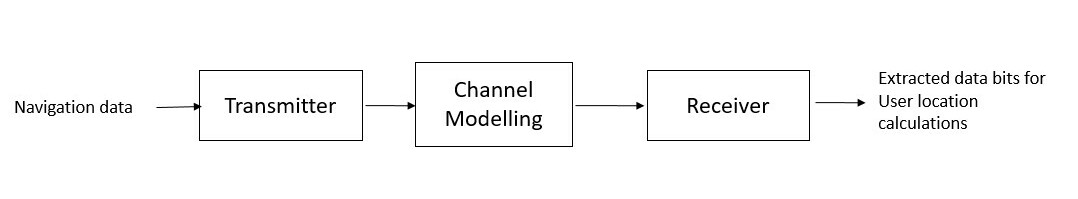
\includegraphics[width=1\columnwidth]{figs/simulation_overview.jpg}
\centering
\captionsetup{justification=centering}
\caption{Transmitter Block diagram}
\label{fig:sim_flow}
\end{figure}


Navigation data is randomly generated and subframes and master frames are created as per the frame structure described earlier. The transmitter module creates the required baseband signal as per the modulation scheme, with relevant channel encosing schemes. Channel modelling module adds various modelling parameteers and AWGN noise to the baseband signals for different satellites, forming a composite signal. The receiver module receives the composite signal, processes it to extract the navigation data, that was originally sent.  

\let\cleardoublepage\clearpage
